\subsection{Разработка архитектуры iOS приложения}
\label{sec:development:arch:ios}

Перед описанием финальной архитектуры приложения стоит рассмотреть конкретные технологии, которые будут использоваться на проекте.

\subsubsection{}
\label{sec:development:arch:ios:swift}

\textbf{Swift} -- язык программирования общего назначения, разрабатываемый с современным подходом к безопасности, производительности и паттернам дизайна программного обеспечения\cite{swift:about}. 

Заявлена поддержка платформ компании Apple (iOS, watchOS, tvOS, macOS и любые будущие), Linux и многих других в тестовом режиме. Компиляция происходит при помощи \gls{llvm}, поэтому у языка большой потенциал для покорения новых платформ.

Целью проекта Swift является создание языка для использования в различных направлениях: от системного программирования, до мобильных приложений, масштабирующегося до объёмов облачных сервисов. Основные принципы, которыми руководствуются дизайнеры и разработчики языка:

\begin{enumerate}
	\item \emph{Безопасность}. Язык всячески старается избегать неопределённого поведения, снимает с разработчика необходимость беспокоиться о работе с указателями, напрямую с памятью, заставляет обрабатывать (или игнорировать, явно это отмечая) большинство мест, уязвимых для ошибок разработчиков.
	\item \emph{Скорость}. Язык предполагается как альтернатива языкам, основанным на C(C, C++, Objective-C), что автоматически поднимает вопрос его способности составить им конкуренцию в производительности. Swift держит высокую планку предсказуемой производительности (нет неожиданных понижений производительности на различные процессы языка и \gls{sdk}, например нет \gls{gc}).
	\item \emph{Выразительность}. Swift использует десятилетия достижений в Информатики, предоставляя синтаксис, который приносит удовольствие при разработке и чтении, поставляя современные возможности.  
\end{enumerate}

Язык обладает многими возможностями, которые упрощают написание и чтение кода, по прежнему предоставляя разработчику контроль, необходимый для системного программирования. Swift поддерживает вывод типов, модульность, управление памятью является автоматическим, неполный список особенных и отлично реализованных возможностей языка:

\begin{itemize}
	\item замыкания, унифицированные для совместного использования с указателями на функции;
	\item множественные возвращаемые результаты из функций, поддержка Tuples на уровне языка;
	\item обобщения;
	\item гибкие структуры, поддерживающие методы, расширения и протоколы;
	\item паттерны мира функционального программирования;
	\item эффективная система обработок ошибок, интегрированная в систему типов;
	\item паттерн матчинг;
	\item продвинутые механизмы для контроля потока выполнения;
	\item неизменяемые переменные и типы данных;
	\item optional и набор синтаксического сахара для удобной работы с ним.
\end{itemize}

Язык является компилируемым, имеет поддержку \textit{REPL}, расширяет стандартный подход к использованию \gls{llvm} (компиляция производится в два этапа в \textit{SIL}, \textit{LLVM IR}, с набором оптимизаций на каждом).

В языке широко используется парадигма \textit{Value Type}, которая разделяет все типы на ссылочные и типы значений. Типы значений передаются в методы по значению (копируются), ссылочные -- по ссылке. Копирование значения позволяет разработчику меньше беспокоиться о непредвиденных мутациях данных, одновременном доступе к данным с разных потоков.

Частью языка является оптимизация \gls{cow}, копирующая значения только при их непосредственном изменении. Оптимизация отлично сочетается с типами значений, позволяя сохранить производительность ссылочных типов. Механизм достаточно умён для определения одинаковых значений, что позволяет не выделять место для изменённых данных, если в памяти уже имеется блок данных с таким же значением. Язык позволяет встроить \gls{cow} в собственные типы данных. При выполнении кода на рисунке \ref{sec:development:arch:ios:swift:code:cow} для переменных x и z не будет аллоцироваться память, а для y -- будет.

\begin{figure}[h]
	\lstinputlisting{inc/src/swift_cow_example.swift}
   \caption{Пример кода, подлежащего COW оптимизации}
   \label{sec:development:arch:ios:swift:code:cow}
\end{figure}

В языке поддерживаются два вида алгебраических типов данных:

\begin{enumerate}
	\item \emph{Sum Types} (тип-сумма). Типы данных, все возможные значения которых вычисляются путём \textit{суммирования} количества всех возможных значений внутренних типов данных.
	\item \emph{Product Types} (тип-произведение). Типы данных, все возможные значения которых вычисляются путём получения мощности \textit{декартового произведения} всех возможных значений внутренних типов данных.
\end{enumerate}

Примерами типов-произведения являются структуры и классы, типов-суммирования -- \textit{Tuple} и перечисления. Язык имеет мощную систему перечислений, позволяющую установить взаимное соответствие между элементами перечисления и значениями любого типа, задать каждому элементу перечисления набор ассоциированных значений. Пример типа-суммы представлен на рисунке \ref{sec:development:arch:ios:swift:code:barcode}.

\begin{figure}[h]
	\lstinputlisting{inc/src/swift_enum_sample.swift}
   \caption{Пример типа-суммы в Swift}
   \label{sec:development:arch:ios:swift:code:barcode}
\end{figure}
\subsubsection{}
\label{sec:development:arch:ios:rxswift}

\textbf{RxSwift} -- имплементация библиотеки ReactiveX, рассмотренной в~пункте \ref{sec:analysis:research:mobArch:rx}. Фреймворк является не единственной попыткой портировать идеи \gls{rx} на~платформу iOS, но~имеет большое количество достоинств перед альтернативами:

\begin{itemize}
	\item разработан на~языке Swift;
	\item придерживается конвенций ReactiveX;
	\item реализует несколько уточнённых версий \gls{observable}: \textit{Single}, \textit{Maybe};
	\item имеет поддежку connectable \gls{observable};
	\item частью поставки RxSwift является библиотека RxCocoa, предоставляющая реактивный \gls{api} для~многих стандартных контролов и~классов;
	\item унифицировано оборачивает механизмы системы(Delegate Proxy, KVO, Notifications);
	\item имеет расширяемый набор планировщиков, позволяющих использовать libDispatch и~NSOperationQueue.
\end{itemize}
\subsubsection{}
\label{sec:development:arch:ios:realm}

\emph{Realm} --- система управления базой данных, нацеленная на использованияе в приложениях для мобильных устройств(Android, iOS, Xamarin, React Native). Дизайн базы использует парадигму реактивного программирования, многие классы являются <<живыми>>: обновляются вместе с изменением базы и способны высылать уведомления об изменившихся данных. К основным особенностям Realm можно отнести:

\begin{itemize}
	\item работа с базой происходит с использованием моделей, написанных разработчиком на привычном языке программирования;
	\item данные хранятся в бинарном формате, схемой для которого выступают классы-модели;
	\item база поддерживает связи один к одному, один ко многим, создание связи между типами автоматически создаёт обратную связь;
	\item поддержка индексируемых полей;
	\item поддержка первичных ключей;
	\item частичная поддержка NSPredicate на iOS;
	\item организация ленивого чтения из базы при помощи прокси-объектов, что с одной стороны позволяет использовать API так, будто чтение не является ленивым, а с другой -- обойтись без лишних вычислений;
	\item реактивный подход, который выражен в виде <<живых>> запросов, объектов и возможности получать уведомления об изменениях данных (на iOS существует интеграция с \gls{kvo});
	\item <<точные уведомления>> -- механизм Realm, позволяющий вместе с уведомлением об изменениях получить список изменений, адаптированный для обновления UI-коллекций;
	\item потокобезопасность.
\end{itemize}

Существует большое количество сторонних библиотек, использующих расширяющих Realm, на проекте используются:

\begin{itemize}
	\item \emph{RxRealm} -- обёртка над \gls{api} Realm, позволяющая превращать объекты и запросы в \gls{observable} и описывающая операции записи/удаления в виде \gls{observable};
	\item \emph{RxRealmDataSources} -- адаптер Realm для механизма биндинга данных к UI-коллекциям, реализованном в RxCocoa.
\end{itemize}
\subsubsection{}
\label{sec:development:arch:ios:rxfeedback}

Многие процессы можно органично описать в виде \gls{observable}, однако бывают случаи, когда процесс является непрерывным и интерактивным длительное время, требует промежуточного сохранения состояния. Специально для построения реактивных систем с мемоизацией состояния и наличием обратной связи был разработан паттерн \emph{RxFeedback}, который будет рассмотрен далее.

Частым решением является по прежнему описывать операцию в виде потока (например, запрос в сеть), сохранить его результат в обычную переменную (производя правильные синхронизации потоков при чтении/записи) и дальнейшем использовании этого значения для создания новых \gls{observable}. Подход плох необходимостью разрывать поток и постоянной заботой о проблемах синхронизации. За время разработки приложения появился паттерн, который отлично ложился в дизайн большинства модулей, не связанных с пользовательским интерфейсом.
Самым простым способом рассмотреть подход является решение проблемы, для иллюстрации паттерна я выбрал проблему постраничного запроса данных из сети (получение поисковых результатов из \gls{api} GitHub).

Github возвращает результат поиска в виде списка подходящих под запрос сущностей и опциональной ссылки на следующую страницу. Следовательно, когда от пользователя поступит запрос на получение следующей страницы -- приложению потребуется забрать результат прошлого поиска, вычислить адрес для новой страницы результатов и отправить запрос (точнее делегировать запрос одному из доступных воркеров). Также система должна быть способна уведомить UI об изменениях, статусе выполнения запроса, отбрасывать пользовательские действия, ведущие к старту уже выполняющегося запроса.
Одним из нескольких элементов архитектуры является состояние. Во время разработки стало очевидно, что состояние должно хранить в себе всю информацию (как данные, так и утилитарную), поэтому состояние поиска можно представить в виде листинга \ref{sec:development:arch:ios:rxfeedback:example:state}.

\begin{code}
  \lstinputlisting{inc/src/rx-feedback-state.swift}
   \caption{Пример состояния паттерна RxFeedback}
   \label{sec:development:arch:ios:rxfeedback:example:state}
\end{code}

Второй составляющей является набор событий (по своей сути, у системы есть набор входящих данных - события и выходящих - вычисление обновлённого состояния), к ним можно отнести:

\begin{itemize}
  \item пользователь запросил новые данные;
  \item получен очередной результат поиска;
  \item получена ошибка при выполнении запроса.
\end{itemize}

Часто результаты операций упаковываются в тип Result, позволяя группировать входящие сообщения и типизировать ошибку, однако для простых примеров бывает удобнее разнести успешный результат выполнения операции и ошибку на два разных события. В листинге \ref{sec:development:arch:ios:rxfeedback:example:event} представлен пример описания входящих событий. Чаще всего они описываются в виде перечисления.

\begin{code}
  \lstinputlisting{inc/src/rx-feedback-event.swift}
   \caption{Пример события паттерна RxFeedback}
   \label{sec:development:arch:ios:rxfeedback:example:event}
\end{code}

Следующей компонентой является тип, чья обязанность объяснить системе как изменять состояние для каждого конкретного события. Обычно это тип, который имеет метод \texttt{func create(input: Input) -> (State) -> State}, принимающий событие и возвращающий метод, каким-то образом модифицирующий состояние. Такой подход позволяет создать много небольших чистых функций, которые принимают состояние, определённым образом его меняют и возвращают результат. Часто для модификации состояния используются линзы, позволяя сделать тип состояния полностью неизменяемым, но они не являются обязательными для имплементации паттерна, поэтому я не буду их использовать в примерах. В листинге \ref{sec:development:arch:ios:rxfeedback:example:mutator} приведён пример обработки одного события. Оператор \(>>>\) является композицией функций, метод resetLoopVariables необходим для поддержания консистентного состояния между вызовами (очищает переменные, которые используются для одноразовой передачи данных).

\begin{code}
  \lstinputlisting{inc/src/rx-feedback-state-mutator.swift}
   \caption{Пример события паттерна RxFeedback}
   \label{sec:development:arch:ios:rxfeedback:example:mutator}
\end{code}

Имея данный набор компонент уже можно собрать систему, однако для её корректной работы необходимы сущности, выполняющие работу по запросу из состояния. Обычно такие сущности внедряются при помощи \gls{di} в тип RxFeedback, в нашем случае необходима сущность, способная отправлять запросы в \gls{api} GitHub по требованию, представленная в листинге \ref{sec:development:arch:ios:rxfeedback:example:worker}. В листинге тип возвращает \texttt{Observable<Event>}, но обычно возвращается \texttt{Observable<Result<Event, Error> >}.

\begin{code}
  \lstinputlisting{inc/src/rx-feedback-worker.swift}
   \caption{Пример Worker паттерна RxFeedback}
   \label{sec:development:arch:ios:rxfeedback:example:worker}
\end{code}

Для имплементации остаётся только объединить созданные ранее компоненты, что б получить следующий поток:

\begin{itemize}
  \item тип имеет вход вида \texttt{Any\gls{observer}<Event>};
  \item все сообщения приводятся к одной последовательной очереди;
  \item входящее сообщение превращается в функцию изменения состояния;
  \item функция применяется к предыдущему состоянию;
  \item результат является новым состоянием и доступен всем подписчикам;
  \item тип, отвечающий за выполнение работы оповещается о новом запросе (если такой имеется);
  \item результат работы возвращается на вход системы.
\end{itemize}

В листинге \ref{sec:development:arch:ios:rxfeedback:example:initial-state} представлена функция для генерации начального состояния системы, а в листинге \ref{sec:development:arch:ios:rxfeedback:example:composition} все компоненты связываются в единый поток.

\begin{code}
  \lstinputlisting{inc/src/rx-feedback-initial-state.swift}
   \caption{Начальное состояние для паттерна RxFeedback}
   \label{sec:development:arch:ios:rxfeedback:example:initial-state}
\end{code}

\begin{code}
  \lstinputlisting{inc/src/rx-feedback-composition.swift}
   \caption{Организация потока паттерна RxFeedback}
   \label{sec:development:arch:ios:rxfeedback:example:composition}
\end{code}

Все листинги в этом разделе были приведены в качестве примеров, в настоящей реализации следует обрабатывать ошибки, использовать линзы, Result, правильно проектировать состояние (например, постоянное копирование больших структур сильно замедляет работу приложения).

\FloatBarrier
\subsubsection{}
\label{sec:analysis:research:mobArch:ufeature}

По своей сути приложения состоят из набора функциональных возможностей. Обычно все возможности приложения реализованы в пределах одного модуля. Результатом такого подхода является тесная связанность разных модулей, введение неявных зависимостей, увеличение сложности поддержки и разработки новых функций. Паттерн \gls{mvvm} предназначен для организации пользовательского интерфейса приложения, однако часто приложение можно условно разбить на несколько независимых доменов -- обычно каждый такой домен называется микросервисом.

Микросервисы предоставляют минимальный, но необходимый для интеграции \gls{api}, скрывая детали реализации. Для примера в iOS клиенте чата можно выделить следующие домены:

\begin{itemize}
	\item сервисы для шифрования сообщений, общения с сервером, работой с базой;
	\item экраны списка контактов, настроек, списка диалогов и конкретного диалога.
\end{itemize}

В 2016 году компания SoundCloud представила своё видение организации микросервисной архитектуры в мобильных приложениях: \glspl{ufeature}.

\glspl{ufeature} -- архитектурный подход для стуктурирования iOS приложений, предоставляющий масштабируемость, оптимизацию времени сборки проетка и циклов тестирования, гарантирующий адоптацию хороших практик разработки в команде. Основной идеей подхода является разработка независимых возможностей приложения, которые взаимодействуют при помощи чётко обозначенного \gls{api}\cite{soundcloud:ufeature}.

Типичная \gls{ufeature} представляет из себя отдельный проект с 4 схемами:

\begin{itemize}
	\item код и ресурсы;
	\item тесты;
	\item данные, которые используются в тестах и приложении-примере;
	\item приложение-пример.
\end{itemize}

На рисунке \ref{sec:analysis:research:mobArch:ufeature:featureDependencyDiagram} представлена связь схем одного модуля \gls{ufeature}.

\begin{figure}[h]
  \centering
    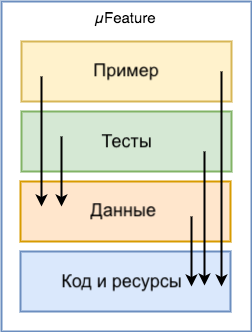
\includegraphics{inc/img/ufeature-diagram.png}
  \caption{Организация схем внутри модуля одной uFeature}
  \label{sec:analysis:research:mobArch:ufeature:featureDependencyDiagram}
\end{figure}

Автор подхода предлагает разделять все \gls{ufeature} на два вида:

\begin{itemize}
	\item \emph{Foundation} -- основные строительные блоки, общие расширение пользовательского интерфейса, сервисы;
	\item \emph{Product} -- возможности, с которыми пользователь взаимодействует и видит на экране, например список диалогов;
\end{itemize}


\subsubsection{}
\label{sec:development:arch:ios:modules}

Финальным пунктом в обзоре архитектуры будущего приложения является выделение основных модулей.

\begin{enumerate}
	
	\item Foundation.Core:
	\begin{enumerate}
		\item Криптография.
		\item База данных.
		\item Веб клиент.
		\item Файловый менеджер.
		\item Менеджер паролей(для работы с KeyChain).
		\item Websocket клиент.
		\item Расширения сторонних библиотек, например RxSwift.
	\end{enumerate}

	\item Foundation.UI:
	\begin{enumerate}
		\item Имплементация MVVM, биндингов.
		\item Переиспользуемые контролы приложения.
		\item Расширения стандартной и сторонних библиотек пользовательского интерфейса, например RxCocoa, UIKit.
		\item Наборы стилей, шрифтов, цветов и ресурсов.
		\item Строки локализации.
	\end{enumerate}

	\item Product.Authorization:
	\begin{enumerate}
		\item Все экраны авторизации.
		\item Модуль авторизации, который предсавляет из себя граф состояний авторизации и рёбра переходов.
		\item \gls{observable} текущего состояния авторизации и данных пользователя.
		\item Веб клиент, имплементирующий \gls{api} атворизации.
		\item Декоратор стандартного веб клиента и websocket клиента, интегрирующий авторизацию в отправляемые запросы.
		\item Декораторы для остальных сервисов, требующих авторизации для полноценной работы(база данных, файловое хранилище).
	\end{enumerate}

	\item Product.Contacts:
	\begin{enumerate}
		\item Экран списка контактов и информации по конкретному контакту.
		\item Сервис для работы с базой данных контактов.
		\item Адаптер, обрабатывающий и посылающий сообщения в websocket, связанные с контактами и списком устройств.
	\end{enumerate}

	\item Product.Dialogues:
	\begin{enumerate}
		\item Экран списка диалогов и деталей по конкретному диалогу.
		\item Сервис для работы с базой данных диалогов.
		\item Имплементация веб клиента для работы с \gls{api} списка диалогов.
	\end{enumerate}

	\item Product.Chat:
	\begin{enumerate}
		\item Экран диалога.
		\item Сервис для работы с базой данных сообщений.
		\item Адаптер, обрабатывающий и посылающий сообщения в websocket, связанные с сообщениями.
		\item Имплементация веб клиента для работы с \gls{api} списка сообщений.
	\end{enumerate}

	\item Product.Settings:
	\begin{enumerate}
		\item Экран настроек.
	\end{enumerate}

	\item App --- готовое приложение, в котором кооржинируется настройка и работа всех модулей.

\end{enumerate}

Как видно из этого списка, каждый модуль требует тесного общения с остальными модулями из своего домена, однако паттерны адавтер и декоратор позволят наслаивать возможности на готовые сервисы, не связывая модули друг с другом.

В пунктах \ref{sec:analysis:research:mobArch:mvc} и \ref{sec:analysis:research:mobArch:mvvm} были рассмотренны основные решения для построения архитектуры пользовательского интерфейса в iOS приложениях, а в пункте \ref{sec:analysis:research:mobArch:ufeature} --- способ организации модульного приолжения. За основну архитектуры будущего приложения было принято выбрать модифицированный паттерн \gls{mvvm}, код приложения будет организован в модули, разбитые на несколько git репозиториев. 